\subsubsection{Проектирование структуры базы данных} \hfill

Проектирование схемы БД является очень важным этапом, от которого зависят последующие этапы разработки АИС. Время, затраченное на проектирование схемы БД, обычно окупается высокой скоростью реализации проекта.

На этапе внешнего проектирования связанного с анализом предметной области были выделены объекты, которые должны использоваться для представления предметной области. То есть была проведена предварительная структуризация объектов предметной области: объекты реального мира подверглись классификации, была зафиксирована совокупность подлежащих отображению в БД типов объектов. Для каждого типа объектов были зафиксирована совокупность свойств, посредством которых должны описываться конкретные объекты этого типа в БД, виды отношений (взаимосвязей) между этими объектами. Следующим шагом является решение вопроса, какая информация об объектах должна быть представлена в БД и как ее представить с помощью данных. Сущность инфологического этапа проектирования является установление соответствия между состоянием предметной области, его восприятием и представлением в БД.

На этапе инфологического проектирования используется неформальная модель предметной области: <<сущность -- связь>>. Это модель позволяет моделировать объекты ПО, взаимоотношения объектов. Основное назначение неформальной модели <<сущность -- связь>> является семантическое описание предметной области и представление информации для обоснования выбора видов моделей и структур данных, которые в дальнейшем будут использованы в системе. Для построения модели типа <<сущность -- связь>> используются три основных конструктивных элемента: сущность, атрибут и связь.

\textbf{Сущность} -- собирательное понятие, абстракция реально существующего объекта, процесса или явления, о котором необходимо хранить информацию в системе. В качестве сущности в моделях ПО рассматриваются материальные (сотрудник, справка и т.д.) и не материальные (описание некоторого явления, рефераты научных статей и т.д.) объекты реальной действительности. В моделях ПО типа <<сущность -- связь>> каждая рассматриваемая конкретная сущность является узловой точкой сбора информации об этой сущности. В модели также используется понятие <<экземпляр сущности>>. Тип сущности определяет набор однородных объектов, а экземпляр сущности -- конкретный объект в наборе.

\textbf{Атрибут} -- это поименованная характеристика сущности, которая принимает значение из некоторого множества значений. В модели атрибут выступает в качестве средства, с помощью которого моделируются свойства сущностей. Основное назначение атрибута – описание свойства сущности, а также идентификация экземпляра сущностей.

\textbf{Связь} выступает в модели в качестве средства, с помощью которого представляются отношения между сущностями предметной области. Тип связи рассматривается между типами сущностей, а конкретный экземпляр связи рассматриваемого типа существует между конкретными экземплярами рассматриваемых типов сущностей. При анализе связей между сущностями могут встречаться бинарные (между двумя сущностями), тернарные (между тремя сущностями) и, в общем случае n-арные связи. Может также встречаться унарные (рекурсивные) связи, когда экземпляр определенного типа сущности связан с другим экземпляром той же самой сущности. Наиболее часто встречаются бинарные связи. Для определения характера взаимосвязей между двумя типами сущностей используются прямое и обратное отображения между двумя соответствующими множествами экземпляров сущностей. При проведении классификации видов связей обычно выделяют следующие виды связей: 1:1, 1:M, M:1, M:N.

Инфологическая модель представляется двумя вариантами записи:
\begin{itemize}
\item Спецификационная форма инфологической модели ПО;
\item Графическая диаграмма инфологической модели ПО.
\end{itemize}

\subsubsubsection{Обоснование выбора инструментария проектирования}
Для проектирования даталогической модели был выбран проблемно-ориентированный язык Haskell Persistent, который обладает следующими преимуществами:
\begin{itemize}
\item Интеграция с языком программирования Haskell -- типы БД непосредственно используются в проектируемой программе без ручного кодирования;
\item Автоматические миграции -- если схема БД изменилась во время проектирования, то данный язык предоставляет средства автоматической миграции данных между схемами;
\item Краткая форма записи и текстовый формат. Благодаря спецификационной записи описание схемы базы данных имеют минимальный объем и позволяет использовать все преимущества системы контроля версий и интегрированных систем разработки.
\end{itemize}

\paragraph{Инфологическая модель базы данных} \hfill

В результате анализа предметной области определены сущности, их атрибуты, взаимосвязь между ними и разработана инфологическая модель базы данных.

Схема инфологической модели представлена в графической части дипломной работы на листе «Инфологическая модель базы данных».

\includepdf[pages=3]{A1.pdf}

\paragraph{Описание сущностей и их атрибуты} \hfill

Выделены следующие сущности предметной области. Описание сущностей и атрибутов представлено в таблицах ниже.

Условные обозначения: РК (primary key) – первичный ключ, FK –внутренний ключ.

\begin{table}[h!]
\centering
\caption{Сущность <<Запрос>>}
\label{table:entityQuery}
\begin{tabular}{L{8cm}|L{8cm}}
\multicolumn{1}{C{8cm}|}{Имя атрибута} & 
\multicolumn{1}{C{8cm}}{Описание атрибута} \\
\hline\hline

Код запроса (PK) & Идентифицирующий атрибут \\
Название запроса & Название запроса \\
Альфа-код запроса & Код страны/провинции, описываемой запросом по ISO 3166 \\
Полнотекстовый запрос & Основная часть запроса \\
Дополнительный запрос & Дополнительные фильтры результатов \\
Начальная дата & Минимальная дата результата \\
Конечная дата & Максимальная дата результата  \\
Начальная дата сбора & Минимальная дата сбора результата \\
Конечная дата сбора & Максимальная дата сбора результата \\
Смещение результата & Количество документов, которое следует опустить из результатов \\
Размер страницы & Максимальное количество документов, которое нужно вернуть в результатах \\
Поле сортировки & Поле, по которому следует отсортировать результаты \\
Направление сортировки & Сортировка по убыванию или возрастанию \\
Без меток & Признак поиска только документов без меток \\

\end{tabular}
\end{table}

\begin{table}[h!]
\centering
\caption{Сущность <<Прогноз>>}
\label{table:entityPredict}
\begin{tabular}{L{8cm}|L{8cm}}
\multicolumn{1}{C{8cm}|}{Имя атрибута} & 
\multicolumn{1}{C{8cm}}{Описание атрибута} \\
\hline\hline

Код прогноза (PK) & Идентифицирующий атрибут \\
Сохраненный запрос (FK) & Код сохраненного запроса для прогноза \\
Название & Название прогноза \\
Описание & Описание прогноза \\
Точка отсчета & Начальная точка прогноза \\
Окно обучения & Количество точек от текущей даты для обучения алгоритма \\
Период прогноза & Количество дней в будущее для которого строится прогноз \\

\end{tabular}
\end{table}

\begin{table}[h!]
\centering
\caption{Сущность <<Измерение>>}
\label{table:entityMeasure}
\begin{tabular}{L{8cm}|L{8cm}}
\multicolumn{1}{C{8cm}|}{Имя атрибута} & 
\multicolumn{1}{C{8cm}}{Описание атрибута} \\
\hline\hline

Код измерения (PK) & Идентифицирующий атрибут \\
Прогноз (FK) & Код прогноза, для которого проводилось измерение \\
День & Точка, в которой замерялось значение \\
Значение & Количество результатов по запросу прогноза \\

\end{tabular}
\end{table}

\begin{table}[h!]
\centering
\caption{Сущность <<Популяция>>}
\label{table:entityPopulation}
\begin{tabular}{L{8cm}|L{8cm}}
\multicolumn{1}{C{8cm}|}{Имя атрибута} & 
\multicolumn{1}{C{8cm}}{Описание атрибута} \\
\hline\hline

Код популяции (PK) & Идентифицирующий атрибут \\
Прогноз (FK) & Код прогноза, к которому относится популяция \\
Поколение & Текущий номер поколения популяции \\

\end{tabular}
\end{table}

\begin{table}[h!]
\centering
\caption{Сущность <<Формула>>}
\label{table:entityFormula}
\begin{tabular}{L{8cm}|L{8cm}}
\multicolumn{1}{C{8cm}|}{Имя атрибута} & 
\multicolumn{1}{C{8cm}}{Описание атрибута} \\
\hline\hline

Код формулы (PK) & Идентифицирующий атрибут \\
Популяция (FK) & Код популяции, к которой относится формула \\
Текст & Текстовое представление формулы \\
Приспособленность & Значение приспособленности формулы \\

\end{tabular}
\end{table}

\begin{table}[h!]
\centering
\caption{Сущность <<Приспособленность>>}
\label{table:entityFittness}
\begin{tabular}{L{8cm}|L{8cm}}
\multicolumn{1}{C{8cm}|}{Имя атрибута} & 
\multicolumn{1}{C{8cm}}{Описание атрибута} \\
\hline\hline

Код приспособленности (PK) & Идентифицирующий атрибут \\
Популяция (FK) & Код популяции, к которой относится формула \\
Лучший & Лучшее значение функции приспособленности \\
Среднее & Среднее значение функции приспособленности \\
Поколение & Значение поколения, для которого производились замеры \\

\end{tabular}
\end{table}

\begin{table}[h!]
\centering
\caption{Сущность <<Полином>>}
\label{table:entityMeasure}
\begin{tabular}{L{8cm}|L{8cm}}
\multicolumn{1}{C{8cm}|}{Имя атрибута} & 
\multicolumn{1}{C{8cm}}{Описание атрибута} \\
\hline\hline

Код полинома (PK) & Идентифицирующий атрибут \\
Прогноз (FK) & Код прогноза, для которого проводилось измерение \\
Параметры & Массив параметров полинома \\
СКО & Среднеквадратичное отклонение на выборке \\

\end{tabular}
\end{table}

\begin{table}[h!]
\centering
\caption{Сущность <<Скользящее среднее>>}
\label{table:entityMeasure}
\begin{tabular}{L{8cm}|L{8cm}}
\multicolumn{1}{C{8cm}|}{Имя атрибута} & 
\multicolumn{1}{C{8cm}}{Описание атрибута} \\
\hline\hline

Код скользящего среднего (PK) & Идентифицирующий атрибут \\
Прогноз (FK) & Код прогноза, для которого проводилось измерение \\
Размер окна & Размер окна скользящего среднего \\
Веса & Массив весов для средневзвешенной суммы \\

\end{tabular}
\end{table}

\begin{table}[h!]
\centering
\caption{Сущность <<Регион>>}
\label{table:entityMeasure}
\begin{tabular}{L{8cm}|L{8cm}}
\multicolumn{1}{C{8cm}|}{Имя атрибута} & 
\multicolumn{1}{C{8cm}}{Описание атрибута} \\
\hline\hline

Код региона (PK) & Идентифицирующий атрибут \\
Название & Название региона \\

\end{tabular}
\end{table}

\begin{table}[h!]
\centering
\caption{Сущность <<Страна>>}
\label{table:entityMeasure}
\begin{tabular}{L{8cm}|L{8cm}}
\multicolumn{1}{C{8cm}|}{Имя атрибута} & 
\multicolumn{1}{C{8cm}}{Описание атрибута} \\
\hline\hline

Код страны (PK) & Идентифицирующий атрибут \\
Регион (FK) & Код региона, в которую входит страна \\
Название & Название страны \\
Альфа-код & Код страны по ISO 3166-1 \\
Контур & GeoJson с описанием границы страны

\end{tabular}
\end{table}

\begin{table}[h!]
\centering
\caption{Сущность <<Провинция>>}
\label{table:entityMeasure}
\begin{tabular}{L{8cm}|L{8cm}}
\multicolumn{1}{C{8cm}|}{Имя атрибута} & 
\multicolumn{1}{C{8cm}}{Описание атрибута} \\
\hline\hline

Код провинции (PK) & Идентифицирующий атрибут \\
Страна (FK) & Код страны, в которую входит провинция \\
Название & Название провинции \\
Альфа-код & Код провинции по ISO 3166-2 \\
Контур & GeoJson с описанием границы провинции

\end{tabular}
\end{table}

\begin{table}[h!]
\centering
\caption{Сущность <<Сценарий>>}
\label{table:entityMeasure}
\begin{tabular}{L{8cm}|L{8cm}}
\multicolumn{1}{C{8cm}|}{Имя атрибута} & 
\multicolumn{1}{C{8cm}}{Описание атрибута} \\
\hline\hline

Код сценария (PK) & Идентифицирующий атрибут \\
Название & Название сценария \\
Содержание & GeoJson, содержащий элементы сценария \\

\end{tabular}
\end{table}

\begin{table}[h!]
\centering
\caption{Сущность <<Аналитическая записка>>}
\label{table:entityMeasure}
\begin{tabular}{L{8cm}|L{8cm}}
\multicolumn{1}{C{8cm}|}{Имя атрибута} & 
\multicolumn{1}{C{8cm}}{Описание атрибута} \\
\hline\hline

Код записки (PK) & Идентифицирующий атрибут \\
Название & Название аналитической записки \\
Содержание & Содержание записки \\

\end{tabular}
\end{table}

\clearpage
\clearpage
\paragraph{Связи между сущностями} \hfill

Рассмотрим связи между сущностями, выделенными и описанными выше. На основе взаимодействия сущностей в предметной области определим отношения между ними и запишем в таблицу~\ref{table:entityRelations}.

\begin{table}[h!]
\centering
\caption{Связи между сущностями}
\label{table:entityRelations}
\begin{tabular}{C{1cm}|L{6cm}|C{2cm}|L{6cm}}
\multicolumn{1}{C{1cm}|}{№} & 
\multicolumn{1}{C{6cm}|}{Наименование связи} & 
\multicolumn{1}{C{2cm}|}{Тип связи} & 
\multicolumn{1}{C{6cm}}{Сущность} \\
\hline\hline

1 & Берет данные из & M:1 & Прогноз -- Запрос \\
2 & Вычисляется с помощью & M:1 & Измерение -- Прогноз \\
3 & Прогнозирует & M:1 & Популяция -- Прогноз \\
4 & Включается в популяцию & M:1 & Формула -- Популяция \\
5 & Хранит историю о & M:1 & Приспособленность -- Популяция \\
6 & Прогнозирует & M:1 & Полином -- Прогноз \\
7 & Прогнозирует & M:1 & Скользящее среднее -- Прогноз \\
7 & Входит в & M:1 & Страна -- Регион \\
7 & Входит в & M:1 & Провинция -- Страна \\

\end{tabular}
\end{table}

\paragraph{Даталогическая модель данных} \hfill

Для разработки даталогической модели данных была проведена ручная операция перевода инфологической модели в проблемно-ориентированный язык Haskell Persistent. В результате была получена схема даталогической модели данных, представленная в графической части работы.

Проблемно-ориентированный язык Haskell Persistent автоматически генерирует скрипт на языке SQL для создания всех таблиц, отношений и ограничений в БД, а также проводит миграции данных между разными версиями даталогической модели данных при спиральной разработке приложения.

Схема даталогической модели представлена в графической части дипломной работы на листе «Даталогическая модель базы данных».

\includepdf[pages=4]{A1.pdf}

\clearpage
\lstset{caption={Даталогическая модель данных на языке Haskell Persistent},label=PersistentModel}
\lstinputlisting{design/model.persist}

\begin{table}[h!]
\centering
\caption{Таблица <<saved\_query>>}
\label{table:savedQueryDatalog}
\begin{tabular}{L{4cm}|L{4cm}|L{4cm}|L{4cm}}
\multicolumn{1}{C{4cm}|}{Имя поля} & 
\multicolumn{1}{C{4cm}|}{Тип данных} &
\multicolumn{1}{C{4cm}|}{Свойства поля} &
\multicolumn{1}{C{4cm}}{Имя атрибута} \\
\hline\hline

id               & bigint            & not null, PK & Код запроса \\
name             & character varying & not null & Название запроса \\
alpha            & character varying & not null & Альфа-код запроса \\
full\_text\_query  & character varying &  & Полнотекстовый запрос \\
additional\_query & character varying &  & Дополнительный запрос \\
begin\_date       & date              &  & Начальная дата \\
end\_date         & date              &  & Конечная дата \\
begin\_crawl\_date & date              &  & Начальная дата сбора \\
end\_crawl\_date   & date              &  & Конечная дата сбора \\
result\_offset    & bigint            &  & Смещение результата \\
result\_page\_size & bigint            &  & Размер страницы \\
sort\_field       & character varying &  & Поле сортировки \\
sort\_dir         & boolean           &  & Направление сортировки \\
no\_tags          & boolean           & not null & Без меток \\

\end{tabular}
\end{table}

\begin{table}[h!]
\centering
\caption{Таблица <<predict>>}
\label{table:predictDatalog}
\begin{tabular}{L{4cm}|L{4cm}|L{4cm}|L{4cm}}
\multicolumn{1}{C{4cm}|}{Имя поля} & 
\multicolumn{1}{C{4cm}|}{Тип данных} &
\multicolumn{1}{C{4cm}|}{Свойства поля} &
\multicolumn{1}{C{4cm}}{Имя атрибута} \\
\hline\hline

id             & bigint            & not null, PK & Код прогноза \\
saved\_id      & bigint            & not null, FK & Сохранённый запрос \\
name           & character varying & not null & Название  \\
descr          & character varying & not null & Описание \\
origin         & date              & not null & Точка отсчёта \\
predict\_window & bigint            &  & Окно обучения \\
predict\_target & bigint            &  & Период прогноза \\

\end{tabular}
\end{table}

\begin{table}[h!]
\centering
\caption{Таблица <<measure>>}
\label{table:measureDatalog}
\begin{tabular}{L{4cm}|L{4cm}|L{4cm}|L{4cm}}
\multicolumn{1}{C{4cm}|}{Имя поля} & 
\multicolumn{1}{C{4cm}|}{Тип данных} &
\multicolumn{1}{C{4cm}|}{Свойства поля} &
\multicolumn{1}{C{4cm}}{Имя атрибута} \\
\hline\hline

id      & bigint & not null, PK & Код измерения \\
predict & bigint & not null, FK & Прогноз \\
day     & date   & not null & День \\
value   & bigint & not null & Значение \\

\end{tabular}
\end{table}

\begin{table}[h!]
\centering
\caption{Таблица <<population>>}
\label{table:populationDatalog}
\begin{tabular}{L{4cm}|L{4cm}|L{4cm}|L{4cm}}
\multicolumn{1}{C{4cm}|}{Имя поля} & 
\multicolumn{1}{C{4cm}|}{Тип данных} &
\multicolumn{1}{C{4cm}|}{Свойства поля} &
\multicolumn{1}{C{4cm}}{Имя атрибута} \\
\hline\hline

id         & bigint & not null, PK & Код популяции \\
predict    & bigint & not null, FK & Прогноз \\
generation & bigint & not null & Поколение \\

\end{tabular}
\end{table}

\begin{table}[h!]
\centering
\caption{Таблица <<formula>>}
\label{table:formulaDatalog}
\begin{tabular}{L{4cm}|L{4cm}|L{4cm}|L{4cm}}
\multicolumn{1}{C{4cm}|}{Имя поля} & 
\multicolumn{1}{C{4cm}|}{Тип данных} &
\multicolumn{1}{C{4cm}|}{Свойства поля} &
\multicolumn{1}{C{4cm}}{Имя атрибута} \\
\hline\hline

id         & bigint            & not null, PK & Код формулы \\
text       & character varying & not null & Текст \\
fittness   & double precision  & not null & Приспособленность \\
population & bigint            & not null, FK & none \\


\end{tabular}
\end{table}

\begin{table}[h!]
\centering
\caption{Таблица <<fittness>>}
\label{table:fittnessDatalog}
\begin{tabular}{L{4cm}|L{4cm}|L{4cm}|L{4cm}}
\multicolumn{1}{C{4cm}|}{Имя поля} & 
\multicolumn{1}{C{4cm}|}{Тип данных} &
\multicolumn{1}{C{4cm}|}{Свойства поля} &
\multicolumn{1}{C{4cm}}{Имя атрибута} \\
\hline\hline

id         & bigint           & not null, PK & Код приспособленности \\
population & bigint           & not null, FK & Популяция \\
best       & double precision & not null & Лучший \\
average    & double precision & not null & Среднее \\
generation & bigint           & not null & Поколение \\


\end{tabular}
\end{table}

\begin{table}[h!]
\centering
\caption{Таблица <<polynom>>}
\label{table:polynomDatalog}
\begin{tabular}{L{4cm}|L{4cm}|L{4cm}|L{4cm}}
\multicolumn{1}{C{4cm}|}{Имя поля} & 
\multicolumn{1}{C{4cm}|}{Тип данных} &
\multicolumn{1}{C{4cm}|}{Свойства поля} &
\multicolumn{1}{C{4cm}}{Имя атрибута} \\
\hline\hline

id      & bigint            & not null, PK & Код полинома \\
predict & bigint            & not null, FK & Прогноз \\
thetas  & character varying & not null & Параметры \\
mse     & double precision  & not null & СКО \\


\end{tabular}
\end{table}

\begin{table}[h!]
\centering
\caption{Таблица <<w\_m\_a>>}
\label{table:wmaDatalog}
\begin{tabular}{L{4cm}|L{4cm}|L{4cm}|L{4cm}}
\multicolumn{1}{C{4cm}|}{Имя поля} & 
\multicolumn{1}{C{4cm}|}{Тип данных} &
\multicolumn{1}{C{4cm}|}{Свойства поля} &
\multicolumn{1}{C{4cm}}{Имя атрибута} \\
\hline\hline

id           & bigint            & not null, PK & Код скользящего среднего \\
predict      & bigint            & not null, FK & Прогноз \\
window\_size & bigint            & not null & Размер окна \\
weights      & character varying & not null & Веса \\

\end{tabular}
\end{table}


\begin{table}[h!]
\centering
\caption{Таблица <<region>>}
\label{table:regionDatalog}
\begin{tabular}{L{4cm}|L{4cm}|L{4cm}|L{4cm}}
\multicolumn{1}{C{4cm}|}{Имя поля} & 
\multicolumn{1}{C{4cm}|}{Тип данных} &
\multicolumn{1}{C{4cm}|}{Свойства поля} &
\multicolumn{1}{C{4cm}}{Имя атрибута} \\
\hline\hline

id     & bigint            & not null, PK & Код региона \\
name   & character varying & not null & Название региона \\


\end{tabular}
\end{table}

\begin{table}[h!]
\centering
\caption{Таблица <<country>>}
\label{table:countryDatalog}
\begin{tabular}{L{4cm}|L{4cm}|L{4cm}|L{4cm}}
\multicolumn{1}{C{4cm}|}{Имя поля} & 
\multicolumn{1}{C{4cm}|}{Тип данных} &
\multicolumn{1}{C{4cm}|}{Свойства поля} &
\multicolumn{1}{C{4cm}}{Имя атрибута} \\
\hline\hline

id      & bigint            & not null, PK & Код страны \\
name    & character varying & not null & Название \\
alpha   & character varying & not null & Альфа-код \\
region  & bigint            & not null, FK & Регион \\
geojson & character varying & not null & Контур \\

\end{tabular}
\end{table}

\begin{table}[h!]
\centering
\caption{Таблица <<province>>}
\label{table:provinceDatalog}
\begin{tabular}{L{4cm}|L{4cm}|L{4cm}|L{4cm}}
\multicolumn{1}{C{4cm}|}{Имя поля} & 
\multicolumn{1}{C{4cm}|}{Тип данных} &
\multicolumn{1}{C{4cm}|}{Свойства поля} &
\multicolumn{1}{C{4cm}}{Имя атрибута} \\
\hline\hline

id      & bigint            & not null, PK & Код провинции \\
name    & character varying & not null & Название \\
alpha   & character varying & not null & Альфа-код \\
country & bigint            & not null, FK & Страна \\
geojson & character varying & not null & Контур \\


\end{tabular}
\end{table}

\begin{table}[h!]
\centering
\caption{Таблица <<scenario>>}
\label{table:scenarioDatalog}
\begin{tabular}{L{4cm}|L{4cm}|L{4cm}|L{4cm}}
\multicolumn{1}{C{4cm}|}{Имя поля} & 
\multicolumn{1}{C{4cm}|}{Тип данных} &
\multicolumn{1}{C{4cm}|}{Свойства поля} &
\multicolumn{1}{C{4cm}}{Имя атрибута} \\
\hline\hline

id      & bigint            & not null, PK & Код сценария \\
name    & character varying & not null & Название \\
geojson & character varying & not null & Содержание \\


\end{tabular}
\end{table}

\begin{table}[h!]
\centering
\caption{Таблица <<article>>}
\label{table:articleDatalog}
\begin{tabular}{L{4cm}|L{4cm}|L{4cm}|L{4cm}}
\multicolumn{1}{C{4cm}|}{Имя поля} & 
\multicolumn{1}{C{4cm}|}{Тип данных} &
\multicolumn{1}{C{4cm}|}{Свойства поля} &
\multicolumn{1}{C{4cm}}{Имя атрибута} \\
\hline\hline

id      & bigint            & not null, PK & Код записки \\
name    & character varying & not null & Название \\
mdtext & character varying & not null & Содержание \\

\end{tabular}
\end{table}